\documentclass[sigconf]{acmart}
\settopmatter{printacmref=false} % Removes citation information below abstract
\renewcommand\footnotetextcopyrightpermission[1]{} % removes footnote with conference information in first column
\pagestyle{plain} % removes running headers

\usepackage{booktabs} % For formal tables
\usepackage{graphicx} % Required for including images
\graphicspath{{figures/}} % Location of the graphics files
\usepackage{booktabs} % Top and bottom rules for table
\usepackage[font=small,labelfont=bf]{caption} % Required for specifying captions to tables and figures
\usepackage{amsfonts, amsmath, amsthm, amssymb} % For math fonts, symbols and environments
\usepackage{wrapfig} % Allows wrapping text around tables and figures
\usepackage{hyperref}
\usepackage{multirow}
\usepackage{rotating}
% \usepackage{subfig}% http://ctan.org/pkg/subfig
\usepackage {tikz}
\usetikzlibrary {positioning}
%\usepackage {xcolor}
\definecolor {processblue}{cmyk}{0.96,0,0,0}
\usepackage{caption}
\usepackage{subcaption}
\usepackage{dblfloatfix}

% \makeatletter
% \def\@copyrightspace{\relax}
% \makeatother

% correct bad hyphenation here
\hyphenation{Page-Rank}

\begin{document}
\title{Information Retrieval on the UCL Website}
\subtitle{COMPGI15}


\author{Minttu Alakuijala}
\affiliation{\institution{}}
\email{minttu.alakuijala.14@ucl.ac.uk}

\author{Nathalie Von Huth}
\affiliation{\institution{}}
\email{nathalie.huth.14@ucl.ac.uk}

\author{Aoi Yamamoto}
\affiliation{\institution{}}
\email{aoi.yamamoto.16@ucl.ac.uk}

\author{Yuechen Zhang}
\affiliation{\institution{}}
\email{yuechen.zhang.16@ucl.ac.uk}

% The default list of authors is too long for headers}
% \renewcommand{\shortauthors}{B. Trovato et al.}


\begin{abstract}

Finding information on the World Wide Web has become of central importance to everyday affairs. Users often have certain needs such as relevancy, speed and accuracy of results. Over the past few decades, ranking algorithms in information retrieval systems have largely shaped not only how we surf the web, but also how we navigate private information such as emails and files in cloud storage. The goal of retrieval systems is to cover the user's needs by providing the most relevant documents given one or multiple search terms. The results need to be fair, justified, and able to capture the intent of the user. This report explores some of the most widely adopted algorithms and measures their performance against an original test set. Based on an index of the UCL Computer Science department domain (cs.ucl.ac.uk), we report results on Boolean retrieval, Term Frequency -- Inverse Document Frequency, BM25 and query likelihood ranking algorithms, each with the added option of including PageRank authority scores. After evaluating our results through precision, recall, F1 and discounted cumulative gain, we concluded that BM25 performs best out of the four ranking algorithms with scores of up to 70\% precision and up to 62\% recall, and managed to outperform the UCL search engine. TF-IDF and query likelihood follow closely behind BM25. It was also observed that for our restricted domain with relatively few internal hyperlinks, PageRank does not add relevance value, as it overemphasises pages with incoming hyperlinks.

\end{abstract}

\maketitle

\section{Introduction}

The end of the 20th century gave rise to a need to quickly obtain information on the World Wide Web. As a result of this, search engines were developed and are one of the most common methods to find information online today. Competition between different search engines has been present since the start, but Google has long ruled the market. Its has become widely used because its algorithms have outperformed those of other search engines. Not all of the algorithms that Google is using are publicly available, but those that are known have been present through decades, such as TF-IDF, BM25, PageRank and query likelihood ranking.

The aim of this report is to explore existing algorithms for information retrieval and how they perform against each other. The search engine was implemented on the "cs.ucl.ac.uk" domain and includes several preprocessing techniques and data transformations. The application includes implementations of several ranking algorithms and an evaluation of the results. The search engine application built for this project can be found on \url{github.com/navohu/IRDM_GROUP27} and has been implemented in Python.\footnote{All instructions for running the application can be found in the README file in the repository.} Initially, our expectations for the project were to produce results that showed the difference of the current working algorithms, as well as an implementation of a deep learning algorithm. Since our project only included a search on the CS website it would imply that the amount of data might not be sufficient for a deep learning approach.



TODO: Our results ... compare the different ranking algorithms with and without PageRank. Explain what metric showed the best results.


This report will first explain different discoveries within the field of information retrieval, followed by an experiment section. This section will explore the methodology of how we created the search engine like setting up an inverted index, programming the crawler and implementing the algorithms. After the methodology section we will introduce the evaluation methods and metrics we used. Finally, we will analyse our results and provide a discussion about the project and its limitations.


\section{Related Work}
Retrieving and ranking results in a search engine can be done through many different algorithms. In this section, we will explore the literature covering two categories of ranking algorithms: probabilistic and non-probabilistic. We will then investigate how the performance of an algorithm is commonly evaluated given a test set. Furthermore, we will review Deep Learning, a new topic that has caught attention within information retrieval, and how it can be used in search engines.

Today, web search is a tool that individuals, universities and businesses use on a daily basis. Many of these retrieval systems fall under traditional information retrieval (IR). The first web search engine was created in 1993, but soon the renowned search engine Google was created by Larry Page and Sergey Brin. The feature that made Google better than its competitors was an algorithm called PageRank introduced by Page in 1998 \cite{brin1998anatomy}. He describes PageRank as "an objective measure of [a website's] citation importance that corresponds well with people's subjective idea of importance." This ranking algorithm is still used by Google today.

Another method of ranking the importance of a website was developed by Kleinberg in 1999 \cite{kleinberg1999authoritative}. He proposed a link analysis algorithm called HITS. It involves identifying hubs and authorities in a web graph, where hubs serve as large directories without specific authoritative information, while authorities hold important information. % TODO: clarify?

Both PageRank and HITS are algorithms that rank the importance of a page, but do not take a query into consideration.
% TODO: clarify the sentence below
Hence, these algorithms are good for ranking the difference between results returned by algorithms that take the query into consideration.
Within query-dependent rankers, one of the earliest and simplest non-probabilistic algorithms was the Standard Boolean model introduced by Fayen \cite{lancaster1973information}. Since this algorithm is based on an exact match between the query terms and the document content, it will often either return too many or too few documents. This simple model was improved upon with more sophisticated algorithms such as the Vector Space Model \cite{salton1975vector}, Term Frequency -- Inverse Document Frequency (TF-IDF) \cite{salton1983mcgill}, and query likelihood language models \cite{zhai2001model} among others. They all have a goal of retrieving the most relevant documents for a given query. \\

IR research has always had a strong emphasis on measuring the efficacy of an IR system. This includes estimating the relevance of documents retrieved by a search engine relative to the user's information need. Evaluation is important in order to assess the performance of the system, measure the differences of multiple systems, and to learn the faults of a system such that IR methods can be improved in the future. The Text Retrieval Conference (TREC) supports and influences the IR community by providing evaluation infrastructure. The famous infrastructure for evaluation, trec\_eval, is used for all ad hoc tasks in TREC \cite{voorhees:evaluation}. Two of its measurements are precision and recall, first developed by Sparck-Jones \cite{jones1981information}. This type of evaluation is based on a document collection that includes documents classified as relevant or non-relevant, based on a set of queries.

On the other hand, work on IR evaluation has shown that defining relevance is very hard when it comes to "real" users \cite{mizzaro1997relevance}. Therefore, another method of capturing user interactions with a search engine is Transaction Log Analysis (TLA). It is based on creating transaction logs to recognise attributes within the search process. It's a way of measuring the searcher's actions, the interaction between the user and the system along with the results \cite{glaser1967discovery}. 

Having a stable and robust test collection is an important part of evaluation. This has resulted in a connected community where researchers have shared test collections with each other. Mark Sanderson emphasises the power of good test collections used in conjunction with evaluation measures \cite{sanderson:evaluation}. Evaluation methods used by Sanderson include Discounted Cumulative Gain (DCG) and normalised DCG (nDCG). DCG is often used to measure the ranking quality and the effectiveness of web-based search engines specifically. The algorithm measures the \textit{gain} of a document based on its position in the list. nDCG normalises the gain across queries, which is done by sorting the relevant documents by their relative relevance.

The very popular subject Deep Learning has also been used in web search engines. Huang, PS. \emph{et al.} proposes a deep structured semantic model that is trained by trying to reach the maximum conditional likelihood of a clicked document given a query \cite{huang2013learning}. The idea is based on click-through data collected which is used to feed the model in order to learn which pages are relevant to a query. Another paper by Deng, L. \emph{et al.} used deep stacking networks (DNS) in order to perform a parallel and scalable relevance prediction on an IR task \cite{deng2013deep}. It outperforms previous well known machine learning ranking algorithms such as LambdaRank and LambdaMART \cite{burges2010ranknet} in normalised DCG. 

Many of these algorithm are commonly used in web search today and the rest of the report will explore how some of these techniques can be used in a search engine. A comparison between different methods will also be provided.


% section related_work (end)


\section{Experiments} % (fold)
\label{sec:experiment}

This section will present the overall methodology of building a search engine. Our methodology is freely and easily adaptable since it uses open source Python libraries and free-tier instances of Amazon Web Services Elastic Compute Cloud (EC2) and Relational Database Service (RDS). There are five main algorithms that have been implemented and contrasted in this project: Boolean Retrieval, TF-IDF, BM25, query likelihood estimation and PageRank. The assortment of algorithms was chosen after a thorough examination of the current literature in the field. We wanted to both test algorithms that have been shown to be very accurate and include some that are less advanced in order to provide a full overview of the the most known algorithms in the field, and cover the main differences between them. 

\subsection{Dataset Description} % (fold)
\label{sub:dataset_description}

The search engine is dealing with two core datasets: the crawled web pages and the test set for evaluation. The crawled web pages are specifically modified and transformed for use. Examples of this include creating an inverted index based on the content of the crawled web pages or producing an adjacency matrix based on the relationship between pages.

The test set was manually created in order for us to evaluate the performance of our search engine. Two main test sets were created: one for precision, and one for recall. This means that one test set is specifically created such that the user want \emph{one} specific document (precision), while the other test set is created to retrieve as many relevant documents as possible (recall). Both test sets needed queries and relevant documents related to the queries. There are also three different types of queries: informational, transactional and navigational queries. The two test sets therefore includes all three types of queries.

% subsection dataset_description (end)

\subsection{Indexing} % (fold)
\label{sub:methods}
A well-designed index is central to search engine performance. Before we could experiment with ranking algorithms, we had to set up cloud computing infrastructure for our index database, define the search domain to crawl, design a database schema and populate it with indexed data. The design decisions we made in the process are highlighted below. %The methodology includes a wide range of steps and exploration in order to build our search engine. These will be presented here.

\subsubsection{AWS Database \& Server Setup} % (fold)
\label{ssub:database_and_server_setup}

The search engine is run on an Amazon EC2 instance that provided secure and resizeable computing capacity. It is usually good practice to run heavy loaded applications -- such as a search engine -- on a cloud computing service. As a rule, there are more computing resources available, and these are more scalable and robust than on a local machine. Another advantage is that it's possible to set up a database instance which can be accessed by anyone. Our project is using a PostgreSQL database within RDS which can be accessed by the search engine running on either the EC2 server or a local machine outside AWS, if needed. However, due to geographical proximity of AWS services, faster performance can be observed from the EC2.\\

%We designed our database schema in such a way that it would be easy for our application to access the data when processing the rankings. To reduce redundancy and the risk of inconsistency, website links, content words and titles are each only stored once and referenced by foreign key IDs in other tables.
We designed our database schema with expandability, consistency, and ease of access in mind. It is mainly made up of tables \emph{cs\_sites}, \emph{cs\_dictionary} and \emph{cs\_word\_occurrence}, prefaced by \emph{cs} to allow further domains to be readily added. Furthermore, the database contains \emph{raw} dictionary and word occurrence tables (with the word \emph{raw} referring to unprocessed document terms), which can be used to isolate the effect of stopping and stemming on the final results.

Our crawler writes to \emph{cs\_cites}, built to hold the titles, URLs and unique IDs of web pages within the CS domain.
Based on these URLs, an inverted index is created, consisting of a dictionary that maps words to their IDs and collection-wide frequencies, and of a word occurrence table, which lists $word\_id$ -- $document\_id$ pairs and their frequencies. After the index is constructed, \emph{cs\_sites} is supplemented with document length and pagerank data.

% subsubsection database_and_server_setup (end)

\subsubsection{Crawling} % (fold)
\label{ssub:crawling}

The crawling was done through an open source platform called Scrapy written in Python.\footnote{https://scrapy.org} This platform is given a start URL "\url{www.cs.ucl.ac.uk}", followed by a depth-first-search on all links containing the "\url{cs.ucl.ac.uk}" domain. This would include pages such as "\url{www.cs.ucl.ac.uk/home}", and "\url{www.wiki.cs.ucl.ac.uk}". We set a \emph{maximum depth} of the crawler because we found some links that were extremely long only contained parts of the internal index of the CS website that were practically never opened by visitors to the website. The crawler also made sure not to crawl already crawled links. In the graph in Figure \ref{fig:graph} we can see an example where some links are pointing back to the root. These links would therefore not be crawled again.

\begin{figure}[!h]
\centering
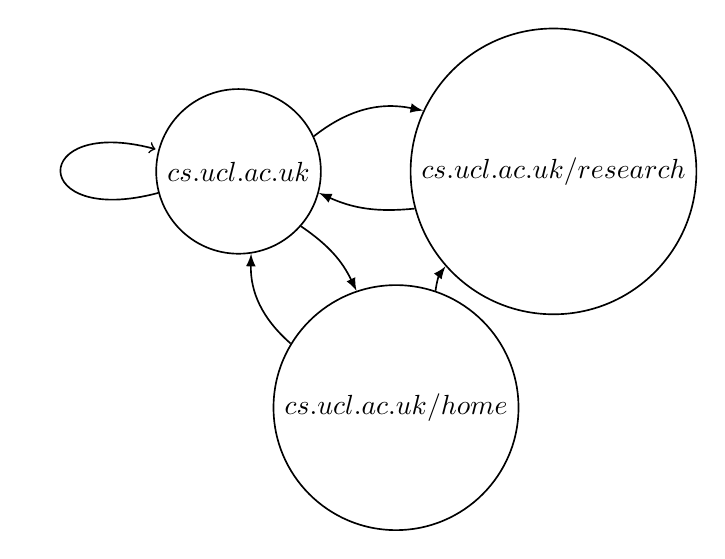
\begin{tikzpicture}[-latex ,auto ,node distance =3cm and 2cm ,on grid ,
                    semithick , state/.style ={ circle ,top color =white , 
                    bottom color = white!20 , draw, black , 
                    text=black , minimum width =1 cm}]
\node[state] (C) {$cs.ucl.ac.uk/home$};
\node[state] (A) [above left=of C] {$cs.ucl.ac.uk$};
\node[state] (B) [above right =of C] {$cs.ucl.ac.uk/research$};
\path (A) edge [loop left] node[left] {} (A);
\path (C) edge [bend left =25] node[below =0.15 cm] {} (A);
\path (A) edge [bend right = -15] node[below =0.15 cm] {} (C);
\path (A) edge [bend left =25] node[above] {} (B);
\path (B) edge [bend left =15] node[below =0.15 cm] {} (A);
\path (C) edge [bend left =15] node[below =0.15 cm] {} (B);
\end{tikzpicture}
\caption{The figure shows a small transition diagram between three websites and how they are related to each other.}
\label{fig:graph}
\end{figure}

The elements that were crawled from the website were the urls, titles ($<$h1$>$ tags) and the anchor text. This information, along with a unique identifier, was stored in the table \emph{cs\_sites}. We didn't crawl and store the content of the pages because of storage limitations. As long as all links of the domain are contained in the database, it is easy to access the content of each page at the indexing stage.

% subsubsection crawling (end)

\subsubsection{Inverted Index} % (fold)
\label{ssub:inverted_index}

To map each word to the IDs of documents it appears in, and then reduce that set of pairs by counting the frequency of each pair, we used Apache Spark, an open-source big data processing framework based on the MapReduce paradigm. In this way, we were able to parallelise the computation-heavy task of retrieving the content of each website, pre-processing its terms and aggregating the results before writing them to the database. We ran Spark on the EC2 server as well as on an Elastic MapReduce cluster with two worker nodes for increased throughput.

%Explain the columns that were added to the cs\_sites table

% subsubsection inverted_index (end)

\subsection{Ranking algorithms}
\label{sub:ranking}

The ranking algorithms we applied on the inverted index can roughly be divided into two categories: standalone rankers and query-insensitive supplementary metrics. In the standalone category, we implemented Boolean retrieval, TF-IDF, BM25 and Query Likelihood ranking. In addition, we added an option to include PageRank scoring to augment the ranking of each of the former algorithms. PageRank itself belongs to the latter supplementary category, since it can not be directly used to retrieve results for a query, as it does not take query terms into consideration and depends on page features only.

All of the standalone algorithms can be run within our app, with or without PageRank. In this way, differences in results returned by the algorithms and their respective ranks can be quickly noticed. A more systematic approach to measure the performance of the different ranking algorithms is through proper evaluation. This is explained in the next section.


\subsubsection{PageRank} % (fold)
\label{ssub:pagerank}

The popular algorithm PageRank was developed by Google for ranking the results within a search engine.\footnote{https://en.wikipedia.org/wiki/PageRank} It is also commonly used for measuring the importance of a website. The algorithm is based on an assumption that more important websites are more likely to be pointed to from other websites.

The algorithm implies that it would need a way of representing connections between web sites. This can easily be done with the aid of an adjacency matrix. Firstly, all the connections needed to be measured, which was done by obtaining all the outgoing links for each site in \emph{cs\_sites}. Now, each link would point to a certain number of outgoing links disregarding whether they were in the \emph{cs.ucl.ac.uk} domain or not, but were filtered to eventually only hold links within the CS domain. From these connections an adjacency matrix was produced as shown as an example in Table \ref{fig:adj_mx}. 

\begin{table}[!h]
  \centering
  \begin{tabular}{|lr|c|c|c|} \cline{3-5}
  \multicolumn{1}{l}{} && \multicolumn{3}{c|}{To} \\ \cline{3-5}
  \multicolumn{1}{l}{} & & A & B & C  \\ \hline
  \multirow{3}{*}{\begin{sideways}From\end{sideways}}
  %                           A   B   C   
  & \multicolumn{1}{|r|}{A} & 0 & 0 & 1  \\ \cline{2-5}
  & \multicolumn{1}{|r|}{B} & 0 & 1 & 1  \\ \cline{2-5}
  & \multicolumn{1}{|r|}{C} & 1 & 1 & 0  \\ \hline
  \end{tabular}
  \caption{Adjacency matrix between links, where A, B and C represents links. The number 1 represents a connection, while 0 represents no connection.}
  \label{fig:adj_mx}
\end{table}

The adjacency matrix was then used in the PageRank algorithm to compute the rank of each link. The implementation would first convert the adjacency matrix into a markov matrix, followed by computing the rank of state \emph{i}:

$$ r_i = r_{i-1} \cdot (I_i *s + S_i * s + T_i * (1-s)) $$ 

where \emph{r} is the PageRank, \emph{$I_i$} is the inlinks of state \emph{i}, \emph{$S_i$} are the sink states, \emph{$T_i$} is the teleporting state and \emph{s} is the probabillity of following a transitions. That means that \emph{s-1} is the probability of teleporting. We have set $s=.85$. The algorithm will continue to calculate \emph{$r_i$} until it reaches a value below the maxerr rate ($maxerr = 0.001$). It is then said to be converged. 

The PageRank is then used in our search engine to rank the differences between similar documents. If two documents showed to have very similar ranks produced, the PageRank weighting can be a useful metric that can give an extra weight to each ranked document. It will then be clearer which documents are more appropriate and most likely more visited. 


% subsubsection pagerank (end)

\subsubsection{Boolean Retrieval} % (fold)
\label{ssub:boolean_retrieval}

Boolean retrieval is a simple ranking algorithm that checks for the presence of query terms in a document. A boolean query can be built up with connectors AND, OR and NOT. All documents that contain terms connected by AND, one or more terms connected by OR, and no terms preceded by NOT, are returned. We implemented Basic Boolean retrieval, in which no distinction in relevance is made between the matching documents. In this model, a document with just one mention of each search term is equally likely to appear at the top of the results as one having a high frequency of the terms. Due to its simplicity, this method serves as a performance baseline to which more advanced algorithms can be compared.

To ensure compatibility between search engine interfaces and comparability of results, we implemented the Basic Boolean model using free text queries instead of a boolean syntax. This means that all natural language queries are considered AND queries. It would not have made sense to compare the results of a "software OR vision AND NOT robot" query to any free text query fed into our remaining models, which is why limiting the connectors to AND is sufficient in this case.
% subsubsection boolean_retrieval (end)

\subsubsection{TF-IDF} % (fold)
\label{sub:tf_idf}

TF-IDF is a type of ranking algorithm that is based off of reflecting how important a certain word is within a document in a collection. Normally, it is used as a weighting factor but can also be used for pure ranking given a query term. It consists of two main concepts:  term frequency (TF) and inverse document frequency (IDF). The two terms have been implemented in the search engine using these equations:

$$TF = \frac{f_{t,d}}{\sum\limits_{t' \in d} f_{t,d}}$$

$$IDF = log_2 \frac{N}{n_t}$$

where $f_{t,d}$ is the number of term occurrences within a document (TF), while the summation is the length of the document. \emph{N} is the number of documents in collection and $n_t$ is the term frequency in the collection. An important notice is that if a term is appearing in more than half of the corpus documents, the IDF would become negative and impossible to interpret against other positive documents. As a result of this drawback we decided to turn all negative values into a small value like $\alpha = 0.001$ in order for the app to compare all the results against each other. All of these terms were retrieved from our database. The documents would then be ranked based on the product of $TF * IDF$ and will display all the documents in descending order. 

% subsection tf_idf (end)

\subsubsection{BM25} % (fold)
\label{ssub:BM25}

BM25 is another type of ranking algorithm developed by Karen Sparck Jones. It is a newer and improved version of TF-IDF. The BM25 belongs to the probabilistic models and uses the "bag of words" concept for retrieving relevant documents from a given search query. The difference from TF-IDF is how BM25 treats the "TF" term. It adjusts the TF score by The formula to adjust the TF score based on the document length is as below where b and k are constants and L is the length of document:

$$ score(D, Q) = \sum_{i=1}^n IDF(q_i) * \frac{f(q_i, D)* (k + 1)}{f(q_i, D) + k * (1-b + b * \frac{|D|}{avgdl})}$$

where the IDF is defined as in subsection \ref{sub:tf_idf}. The same issue with the IDF term turning negative if a term is present in more than half of the document collection also occur for BM25. Hence, the adjustment of setting the IDF term to a small value was also implemented here.

% subsubsection BM25 (end)

\subsubsection{Query Likelihood with Smoothing} % (fold)
\label{ssub:query_likelihood_with_smoothing}

% subsubsection query_likelihood_with_smoothing (end)

% subsection methods (end)

\subsection{Evaluation Metrics} % (fold)
\label{sub:metrics_&_analysis}

The evaluation is an important step to measure performance and will show whether the results of the algorithms conform with expected values. The most common metrics in evaluation within information retrieval is precision, recall and the F1 score. These three are the main evaluation algorithms used within this project. The evaluation is performed on all the ranking algorithms: Boolean retrieval, TF-IDF, BM25 and query likelihood. They are then evaluated in the case of using PageRank and the case without PageRank.

\subsubsection{Queries}
Commonly, there are three types of search query people type into a search engine. These are 'informational queries', 'navigational queries' and 'transaction queries'. 

Informational queries are normally defined as queries that gives the user information about a certain topic, such as a specific place, person, items etc. These queries are normally used when the user is looking for a wider range of information related to the query rather than a specific website. Hence, more relevant documents should be retrieved by the informational queries than the transactional and navigational queries. Our test sets would use 'jun wang' and 'degree' as the informational queries. The reason is that 'jun wang' is more specific than 'degree', therefore we could compare the performances of engines with specific and general queries.

Navigational queries are frequently used when someone is trying to find a certain website or portal. For example, a user might enter 'Facebook' into the search bar to find the Facebook website rather than directly entering the url into the browser's navigational bar. Therefore, the navigational results should be ranked on the top for this kinds of queries. However, some queries that seem to be navigational in nature but might be not. For example, users who search for 'Facebook' might actually be looking for news of Facebook. We decided to use 'Moodle' to represent this kind of queries.

A Transactional query shows an intend to complete a transaction, e.g. making a purchase or paying fees. We skipped this query since there are too few transactional links under the cs.ucl.ac.uk domain. 

\subsubsection{Recall, Precision and F1}
Recall, precision and the F1 score are the most popular metrics to evaluate the performance of a search engine. Precision and recall are both inversely related which means that a high precision will normally give a lower recall and vice versa.

Recall is the ratio between the number of relevant documents retrieved by the search engine and the number of total relevant documents in the database. The formula is shown as below: 

\[recall=\frac{\mid relevant documents\cap retrieved documents\mid}{\mid relevant documents \mid}\]

However, it does not make sense to pursue 100\% recall by returning all documents in response to every query. Therefore, recall alone is not good enough and instead one also needs to measure the non-relevant document retrieved. Precision is a good supplementary metric for exactly this. It measures the ratio between the number of relevant documents retrieved and the total number of document retrieved by the search engine. The formula for precision is shown as below:

\[precision=\frac{\mid relevant documents\cap retrieved documents\mid}{\mid retrieved documents \mid}\]

The F1 score is a good measure of accuracy of the result of the given search engine. It considers both precision and recall of the test to compute the score. The general formula of the F1 score is as follow:

\[F1=(1+\beta^{2})\cdot \frac{precision\cdot recall}{(\beta^{2}\cdot precision)+recall}\]

In our experiment, we would set the parameter to be the traditional value 0.5, and therefore the formula would become this:

\[F1=2\cdot \frac{precision \cdot recall}{precision+recall}\]

\subsubsection{Discounted Cumulative Gain( DCG)}

DCG is a measure of ranking quality. It is used to evaluate the ranking of retrieved documents based on their position in the result list. The gain is accumulated from the top of the list to the bottom with the gain of each result discounted at lower ranks. The higher the DCG value is, the better the ranking is, meaning that more relevant documents are displayed on top of the results list. The formula is as follow:

\[DCG_{k}=\sum_1^k \frac{2^{rel_{i}}-1}{log_{2}(i+1)}\]

% subsection metrics_&_analysis (end)

\subsection{Analysis of Results} % (fold)
\label{sub:analysis_of_results}
Table 2 and 3 indicate the results of average precision, recall and F1 score of tests on algorithms with informational and navigational queries where informational queries include 'degree', 'jun wang' and 'alphago' and navigational queries inlcude 'moodle', 'computer graphical syllabus', 'bioinformatics home page' and 'information retrieval and data mining'  respectively. Algorithms include BM25, QueryLikelihood( QL), Boolean, TF-IDF, BM25 with Pagerank( BM25PG), TF-IDF with Pagerank( TF-IDFPG) and QL with Pagerank. There are totally about 100 links for each query and various number of relevant documents depending on the query.

It can be seen that without consideration of result ranking, the BM25 has the leading performance with both informational and navigational query. This could because that the penalty on term frequency and document length that BM25 implements helps to avoid retrieving non-relevant documents. Also, it strikes to the eyes that algorithms implemented with page ranking are actually worse than them along. One possible reason is that page rank depends on the number of anchors to the objective page, which means the more pages pointing to the objective page, the higher page rank it will receive. However, in our experiment, relevant documents to our queries might not be more popular than the non-relevant ones, therefore the page rank( QLPG) would be a noise while the search engine predicting the relevance. Although more test sets would be required to determine whether the combination is worse than the individual model.

Also, it is interesting to see that the number of recall of results retrieved by navigational queries is generally higher than it of informational queries. This is because that the nature of navigational queries restricts the number of relevant documents. For example, people are just looking for the login page  when they search for moodle and there are nearly no extra information about this term, so the relevant documents would be much fewer than relevant documents of, for example, computer science which is an informational term. Therefore, it is easier for search engine to retrieve most of pages that are relevant to the navigational queries than informational queries.

\begin{table}[H]
\centering
\caption{informational query}

\label{table2}
\resizebox{\columnwidth}{!}{%
\begin{tabular}{|l|l|l|l|l|l|l|l|}
\hline
          & BM25  & QL & TF-IDF &Boolean& BM25PG &QLPG&TF-IDFPG  \\ \hline
Precision & 0.7  & 0.36  & 0.66 & 0.59 &0.52&0.52&0.53 \\ \hline
Recall    & 0.52& 0.49   & 0.51 & 0.5 &0.46&0.48&0.45 \\ \hline
F1 score  & 0.58 & 0.28   & 0.55  & 0.52&0.47&0.49&0.47\\ \hline
\end{tabular}%
}

\end{table}

\begin{table}[H]
\centering
\caption{navigational query}

\label{table2}
\resizebox{\columnwidth}{!}{%
\begin{tabular}{|l|l|l|l|l|l|l|l|}
\hline
          & BM25  & QL & TF-IDF &Boolean& BM25PG &QLPG&TF-IDFPG  \\ \hline
Precision & 0.67  & 0.64  & 0.6 & na  & 0.53 & 0.47 & 0.64 \\ \hline
Recall    & 0.62& 0.57& 0.53& na& 0.5& 0.42& 0.58 \\ \hline
F1 score  & 0.49& 0.44& 47& na& 0.31&0.26 & 0.43\\ \hline
\end{tabular}%
}
\end{table}

Table 3 shows the DCG of performances of each algorithms with different types of queires. BM25 still has significantly better performance than others. We could interpret that BM25 is the best algorithm among those seven. Again, it can be seen that DCG of results from navigational queries is generally higher than informational queries, and hence we can conclude that metrics are also depending on the type of queries rather than algorithm along. Beside, BM25 does not perform well for every search term although it has a better overall performance than other models. For example, For the term bioinformatics, the model BMPG could actually outperform it. Also, for the term alphago, since there are too few of relevant pages, nearly every model could find all of them and put them on the top of the list. 


\begin{table}[H]
\centering
\caption{DCG of models}
\label{my-label}
\resizebox{\columnwidth}{!}{%
\begin{tabular}{|l|l|l|l|l|l|l|l|}
\hline
        & BM25  & QL & TF-IDF & Boolean&BM25PG &QLPG&TF-IDFPG \\ \hline
Informational& 8.57&7.6&7.4&3.9&4.9&5.1&5\\ \hline
navigational& 13.4&10.1&7.4&na&8.6&7.4&10.9\\ \hline
\end{tabular}%
}
\end{table}

\begin{table}[!h]
\centering
\caption{Time of queries with PageRank}
\label{tab:time}
\begin{tabular}{|l|l|}
\hline
        & Avg. Time  \\ \hline
BM25            & 4.619 \\ \hline
QueryLikelihood & 2.109\\ \hline
TF-IDF          & 2.996\\ \hline
\end{tabular}
\end{table}

\begin{table}[!h]
\centering
\caption{Time of queries without PageRank}
\label{tab:time_pr}
\begin{tabular}{|l|l|l|l|}
\hline
        & Avg. Time  \\ \hline
BM25            & 4.012\\ \hline
QueryLikelihood & 1.23\\ \hline
TF-IDF          & 2.109 \\ \hline
\end{tabular}
\end{table}

Another aspect to take into consideration when evaluating performance of an algorithm is the time taken to rank the documents. Table \ref{tab:time} and \ref{tab:time_pr} shows the average time of 10 query words of different lengths, both with and without PageRank. Firstly, we can observe that BM25 spends considerably more time than the others. It is hard to explain the exact reason why it is spending almost double the time, but it might be caused by some implementation issues where for example the database gets called more than usual. Query likelihood seems to perform better than TF-IDF overall as well. It can also be observed a small increase in the timing when applying PageRank to the queries. This can especially be seen for the query likelihood where the time was increased by 42\%.


% subsection analysis_of_results (end)

% section experiment (end)

\section{Discussion \& Limitations} % (fold)
\label{sec:discussion_&_limitations}

Different type of implementation of TF-IDF and BM25, but we have only chosen some. 
Our project has so far only considered a subset of existing algorithms. In order to get a wider picture of the different algorithms, it could be a good idea to include even more ranking algorithms. Also, some additional weighting algorithms could also be included in order to increase the accuracy of our results, such as HITS algorithm.

One of the major limitations in this project was circled around the crawler. The framework Scrapy was not written by us and we would not necessarily know that the crawler did exactly what we asked for. Scrapy retrieved lower amount of pages that expected and therefore made us question its quality. Since this was discovered relatively late, there were no time to try to get used to a new framework. Hence, when analysing the results it must be taken into consideration that the crawler might not have caught all the links in the CS domain. Also the problem with not crawling everything might have been because a max depth was set. Although the crawler indicated that it would take around 20 days without the depth, a further look into improving this should be made.

During the evaluation we had a limitation in our test set. The test set could be increased to compare even more queries, but because of time limitation we were not able to implement any more queries. This limits the credibility of our results, even though they are still sufficient to some extent. For future implementation we would like to implement a Deep Learning task, but because of lack of time and problems of contribution within the team this would be very difficult to finish in time. 

% section discussion_&_limitations (end)

\section{Conclusion} % (fold)
\label{sec:conclusion}

% section conclusion (end)




\bibliographystyle{ACM-Reference-Format}
\bibliography{bibliography} 

\end{document}
